\documentclass[10pt,twocolumn,letterpaper]{article}
%% Welcome to Overleaf!
%% If this is your first time using LaTeX, it might be worth going through this brief presentation:
%% https://www.overleaf.com/latex/learn/free-online-introduction-to-latex-part-1

%% Researchers have been using LaTeX for decades to typeset their papers, producing beautiful, crisp documents in the process. By learning LaTeX, you are effectively following in their footsteps, and learning a highly valuable skill!

%% The \usepackage commands below can be thought of as analogous to importing libraries into Python, for instance. We've pre-formatted this for you, so you can skip right ahead to the title below.

%% Language and font encodings
\usepackage[english]{babel}
\usepackage[utf8x]{inputenc}
\usepackage[T1]{fontenc}

%% Sets page size and margins
\usepackage[a4paper,top=3cm,bottom=2cm,left=3cm,right=3cm,marginparwidth=1.75cm]{geometry}

%% Useful packages
\usepackage{amsmath}
\usepackage{graphicx}
\usepackage[colorinlistoftodos]{todonotes}
\usepackage[colorlinks=true, allcolors=blue]{hyperref}
\usepackage{natbib}
\bibliographystyle{unsrt}
%% Title
\title{
		\usefont{OT1}{bch}{b}{n}
		\normalfont \normalsize \textsc{STEM Fellowship Big Data Challenge 2021 - 2022} \\ [10pt]
		\huge Investigating Renewable Energy Price, Investments, and Technological Innovation to find a solution for the Climate Crisis    \\
}
\selectlanguage{english}
\usepackage{authblk}
\author[]{John Brennan}
\author[]{Michael Perry}
\author[]{Frank Pasztor}
\author[]{Sheldon Broughton}
\affil[]{Neil McNeil Catholic High School}

\begin{document}
\maketitle

\begin{abstract}

Increasing investments in renewable energy will be essential for improving technology innovation and the growth of renewable energy usage and market share. Investments in the newer forms of renewable energy technologies in the areas of solar and wind are strong but these only contain small slivers of the overall energy market. The largest share of the renewal energy share of the market belongs to hydro power. Investment and innovation with hydro power appears to have been flat for some time. We discovered what is taking place with the main sources of renewable energy by analyzing its share of the energy market. Fossil Fuels continue to dominate the energy market  in spite of their negative effects on the environment and human health. On the other hand, renewable energy has captured a significant market share. This share does not appear to be growing. Then we looked at the main types of renewable energy: hydro, solar, and wind. Hydro power has the largest share, then solar and wind. Prices of renewable energy have significantly fallen while volumes of usage have risen. Investments and patents are relatively stable. Therefore, we recommend improved investment, technological innovation, and expansion of the availability of renewable energy. Prices will continue to fall and volumes to increase further, growing the renewables share of the energy market.   


\end{abstract} 

\section*{Keywords}
Renewable Energy, Investments, LCOE, Technology, Innovation 



\section{Introduction}
While it is generally accepted and understood that renewable energy is the way of the future and that it will be essential for the well-being of the planet and human life, we cannot take it for granted. Significant new investments and commitments will be required for progress to be made with renewable energy sources and the expansion of their share of the energy market to replace fossil fuels. Renewable energy is a term for clean, sustainable energy that's derived from naturally regenerating sources. Hydropower is energy that is derived from water and gravity. Solar energy comes from the sun. Wind power comes from objects moved by the wind. These are not completely pure and have environmental and human impacts, but are generally considered superior to the burning of fossil fuels which currently dominates the world’s production of energy. Fossil fuels dominate the global power supply because until very recently electricity from fossil fuels was cheaper and more widely available than electricity from renewable energy sources. This has dramatically changed within the last decade. In most places in the world power from new renewables is now cheaper than power from new fossil fuels. Yet the data that we found shows how new investment and patents in renewable energy may not be as strong as we might expect or desire. Renewable energy will be one of the most important factors in energy security and reducing carbon emissions from fossil fuels and yet the technological innovation and investment activity required to continue growth and improvements are not assured. For the world to transition to low-carbon electricity, energy from these sources needs to be cheaper than electricity from fossil fuels. It is exciting to learn that renewable energy pricing is very competitive with fossil fuels. As Citizens of Earth, we need to start switching from Fossil Fuels to Renewable Energy. These sources, such as the sun and wind, can not be exhausted by us and therefore are called renewable. They cause fewer emissions and are available locally. Their use can, to a large extent, reduce chemical, radioactive, and thermal pollution. They stand out as a viable source of clean and limitless energy. But are we doing enough to move towards renewable energy? While the prices of renewable energy are surprisingly good, investment and commitment need to be improved.  Our Team has discovered that as renewable energy pricing falls, the volume of usage increases. One of the best ways to identify and assess key factors that can change the course of the most dominating energy source is price. The cheaper renewable energy is, the more people around the world have financial access to it. The law of demand states that the quantity purchased varies inversely with price. In other words, the higher the price, the lower the quantity demanded. The lower the price, the higher the quantity demanded. This is an argument for large investments into scaling up renewable energy innovation and production. Increasing installed capacity has the extremely important positive consequence that it drives down the price and thereby makes renewable energy sources more attractive, earlier. In the coming years, most of the additional demand for new electricity will come from low- and middle-income countries; we have the opportunity now to ensure that much of the new power supply will be provided by low-carbon sources. Falling energy prices also mean that the real income of people rises. Investments to scale up energy production with cheap electric power from renewable sources are therefore not only an opportunity to reduce emissions but also to achieve more economic growth – particularly for the poorest places in the world.
The world’s energy supply today is neither safe nor sustainable. With the use of Data Science Algorithms, our team believes that Government and/ or large Corporations' investments should be directed to Renewable Energy Technology. This study is here to prove why directing Government / large Corporation funds towards the production and development of Renewable Energy can drive Renewables to be the Energy Standard. Creating a cleaner safer world, for future generations.
\section*{}



\section{Materials \& Methods}

In our report, we used 10 different Data sets. The software Jupyter was used to graph out all data sets, utilizing the program Python 3, with the libraries of Seaborn, Pandas, Matplotlib, being the fundamental components for our code. The first data set is displaying the data of the World Energy Mix. The data compares the volume of Oil, Gas, Coal, Nuclear, Hydro, Solar, and Wind Energy responsible for part of the Energy Mix. The second data set is comparing the rate of air pollution and deaths that each of the Energy Sources cause. The third data set is comparing the Levelized cost of energy for the three main sources of Renewable Energy (Hydro, Solar, and Wind). The fourth data set is for comparing the main Fossil Fuels index price fluctuations to the Renewable Energy rate of change over the years. The fifth dataset is comparing how much funding has been poured into specific Renewable Energy Technology. The dataset compares the funding between the different types of Renewable Energy Technology. The sixth dataset covers the range of Patents filed for Renewable Technology over the last few decades. Demonstrating the halt in Renewable Technology Innovation, and what changes need to be made to reverse the curve.   


\section{Results}
If Renewable Energy use is going to continue to rise and prices decrease, then there needs to be a renewed focus on investments and technological innovation, focused towards Renewable Energy Technology. 


    % 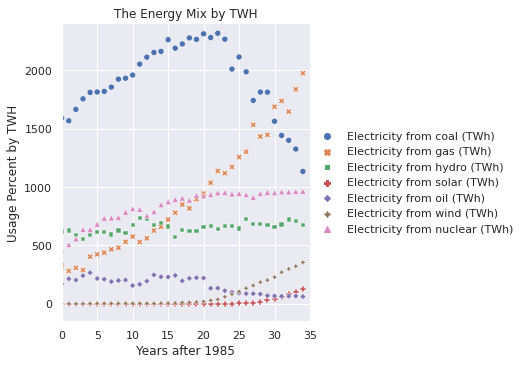
\includegraphics[scale=0.75]{figures/the_energy_mix_by_TWH.PNG}
    % 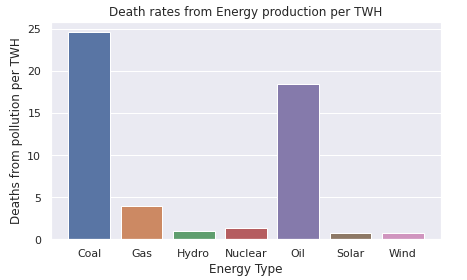
\includegraphics[scale=0.75]{figures/deaths_from_energy.PNG}
    % 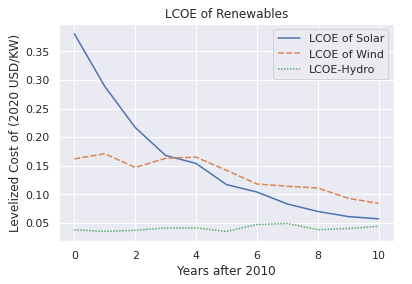
\includegraphics[scale=0.75]{figures/LCOE_of_renewables.PNG}
    % 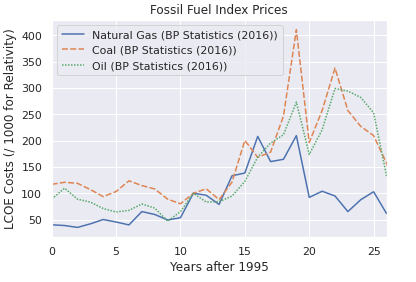
\includegraphics[scale=0.75]{figures/fossil_fuel_index.PNG}
    % 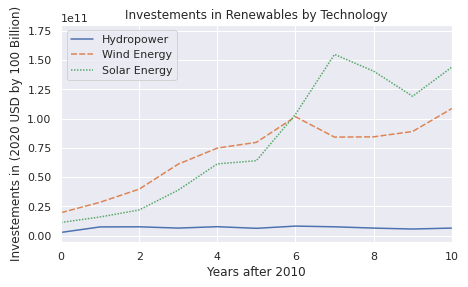
\includegraphics[scale=0.75]{figures/investements_in_renewables.PNG}
    % 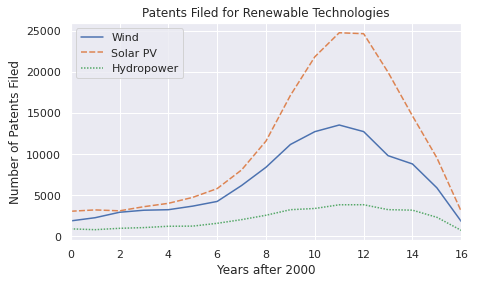
\includegraphics[scale=0.75]{figures/patents_statistics.PNG}


\section{Discussion}



\subsection{The Energy Mix} 

The Energy Mix - As to be expected, the data indicates that fossil fuels continue to dominate the world energy market. However, renewable energy sources have acquired a significant share of the market. 

Since the onset of the Industrial Revolution, the need for ever-larger amounts of inexpensive and accessible energy has been a central concern for modern economies. Vast amounts of energy are required to sustain what we too often take for granted: a stable food supply, comfortable shelter, efficient transportation, and our political, corporate, and social infrastructures. It all depends on the ready availability of energy. Even the technologies that enable this competition to take place, depends on a steady flow of energy from various North American power grids.

As Figure 1 shows, most of this energy continues to come from burning fossil fuels.
Scientific and public concern about the domination of fossil fuels continues to grow as evidence for the deleterious effects of fossil fuels becomes more widely known. Not only do fossil fuels dominate energy usage, but they also dominate the harm caused by energy production as the Death Rates from Energy Production chart shows. The domination of fossil fuels has important implications for the global climate and human health. While numerous scientists express concern that the planet’s earth, air, and water cannot re-absorb the quantities of burned fossil fuels, three-quarters of global greenhouse gas emissions continue to result from the burning of fossil fuels for energy. The world’s electricity supply is dominated by fossil fuels. Coal is by far the biggest source supplying 37\% of electricity; gas is second at 24\%. From “The Energy Mix / Comparing Fossil Fuels and Renewables”

Burning fossil fuels for electricity and heat is the largest single source of global greenhouse gasses, causing 30\% of global emissions. Fossil fuels are responsible for large amounts of local air pollution – a health problem that leads to at least 5 million premature deaths each year. Coal, Gas, and Oil produce the most deaths caused by pollution (see Fig 3). Clearly while fossil fuels – coal, oil, and gas – continue to account for 79\% of the world’s energy production, there is a pressing need for alternative energy sources. There need to be better ways to produce energy than burning stuff. In the charts shown here, we look at the breakdown of renewable technologies by their individual components – hydropower, solar, and wind. It is important to keep in mind that electric energy is only one of several forms of energy that humanity relies on; the transition to low-carbon energy is, therefore, a bigger task than the transition to low-carbon electricity. 

What the above chart on energy safety makes clear is that the alternatives to fossil fuels – renewable energy sources and nuclear power – are orders of magnitude safer and cleaner than fossil fuels. Why then is the world relying on fossil fuels? 

Fossil fuels dominate the world’s energy supply because in the past they were cheaper and more readily available than all other sources of energy. If we want the world to be powered by safer and cleaner alternatives, we have to make sure that those alternatives are cheaper than fossil fuels and more widely available through technological innovation. 

{\scriptsize
\begin{figure}[h!]
    \centering
    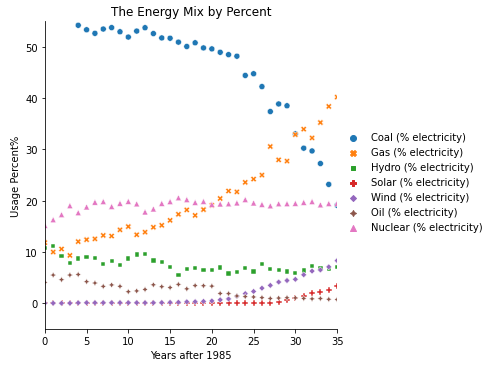
\includegraphics[width=0.6\textwidth]{figures/the_energy_mix_by_percent.PNG}
    \caption{Energy Mix by Percent }

\end{figure}
}

{\scriptsize
\begin{figure}[h!]
    \centering
    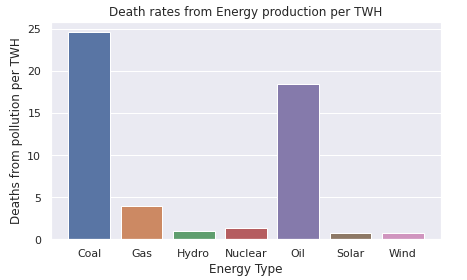
\includegraphics[width=0.6\textwidth]{figures/deaths_from_energy.PNG}
    \caption{Death from Energy Source}

\end{figure}
}



\subsection{Levelized Cost of Energy}

LCOE (Levelized Cost of Energy) and Installed Cost of Renewable Energy - The LCOE of renewable energy sources is experiencing a steadily downward trend at a much faster rate than Fossil Fuels. The cost of solar and wind power is decreasing at a fast pace, whereas hydropower which requires substantial infrastructure investment is steady. 


Figure 3 and 4 here shows how the electricity prices from the long-standing sources of power – fossil fuels and renewable energies – have changed over the last decade. To make comparisons on a consistent basis, energy prices are expressed in ‘Levelized costs of energy (LCOE). One can think of the LCOE from the viewpoint of the manufacturer who builds the Solar Panels. If you are in that situation then the LCOE is the answer to the following question: What would be the minimum price that my customers would need to pay so that the power plant would break even and then make a profit over its lifetime? LCOE takes in the initial cost of building the panels themselves as well as the ongoing costs for electricity to power it and maintenance over its lifetime. 

At US\$0.05/kWh, hydroelectricity remains the lowest-cost source of electricity worldwide, according to a recent report by the International Renewable Energy Agency, entitled Renewable Power Generation Costs in 2017. The global weighted average Levelized cost of electricity from new projects commissioned in 2017 was US\$0.05/kWh from hydropower, compared with US\$0.06 for onshore wind, \$0.07, and \$0.10 for utility-scale solar PV.

Although electricity from hydropower is already cheaper than fossil fuels, the report indicates costs for other renewables should drop, as technology improves. Technological innovation and the subsequent price reductions will result in more new users.  “Electricity from renewables will soon be consistently cheaper than from fossil fuels,” the report says. “By 2020, all the power generation technologies that are now in commercial use will fall within the fossil fuel-fired cost range, with most at the lower end or even undercutting fossil fuels.” 

Despite its positive benefits, hydropower development activity lags that of other renewables. New capacity additions of renewables in 2016 were 162 GW, coming from solar photovoltaic (71 GW), wind (51 GW),  and hydropower (36 GW).
The changes in solar and wind energy costs in recent years are remarkable.  Just 10 years ago it wasn’t even a close race. It was much cheaper to build a new power plant that burns fossil fuels than to build a new solar photovoltaic (PV) or wind plant. On-Short Wind Energy was 22\%, and solar 223\% more expensive than coal.
In the last few years, this has changed entirely.
Electricity from utility-scale solar photovoltaics cost \$359 per MWH in 2009. Within just one decade the price declined by 89\% and the relative price flipped: the electricity price that is needed to reach break-even with the new average coal plant is now much higher than what would be required to build a wind or solar plant.
These rapid price changes represent an important achievement for the alternative energy market and a significant opportunity to capture additional market share. Imagine if some other good had fallen in price as rapidly as renewable electricity: Imagine a customer found a great place to live back in 2010 and at the time they thought it would be worth paying \$4000 in rent. If housing had then seen the price decline that we’ve seen for Solar Energy it would have meant that by 2020 that same customer would be paying only \$300 for the same apartment.
It should be emphasized that it is the relative price that matters for the decision of which type of power plants are built. Did the price decline of renewables matter for the decisions of actual power plant builders in recent years? The simple answer is: Yes it did.
If renewable energy is to resume growing in market share, the price relative to fossil fuels matters. Figure 3 and 4 includes the price of electricity from renewable sources as well the Fossil Fuels Index Prices.



{\scriptsize
\begin{figure}[h!]
    \centering
    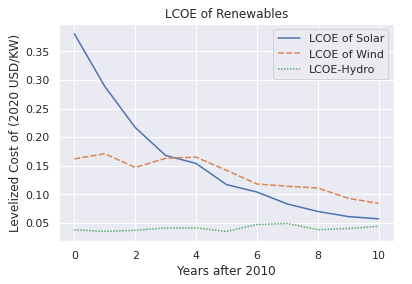
\includegraphics[width=0.6\textwidth]{figures/LCOE_of_renewables.PNG}
    \caption{Cost of Renewables}

\end{figure}
}

{\scriptsize
\begin{figure}[h!]
    \centering
    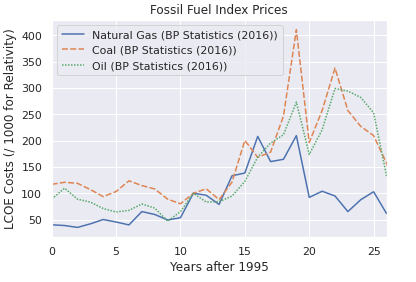
\includegraphics[width=0.6\textwidth]{figures/fossil_fuel_index.PNG}
    \caption{Fossil Fuel Prices}

\end{figure}
}



\subsection{Investments in Renewables}

Investments in Renewables by Technology - Investments in Renewable technology are increasing rapidly. Whereas, hydropower is experiencing little to no new investments streams. While beyond the scope of this paper this is a challenging question that needs to be addressed. Does there need to be a focus on technological innovation or expansion of hydroelectric power? Why is it not seeing significant improvement at this time? Technological innovation and growth do tend to occur in fits and starts rather than in straight lines.

The stability of hydroelectric power also raises the question that perhaps wind and solar are using newer technologies and may also even out in their progress. Solar power investments are increasing quickly. Wind power is also increasing. Investment in hydropower appears to be steady. These questions about the future of renewable energy are vital to human progress in the twenty-first century. The transformation of the global energy system needs to accelerate substantially to meet the objective of the Paris Agreement to limit the rise in average global temperatures to well below 2°C, and ideally to 1.5 °C, by the end of the century, compared to pre-industrial levels. Renewable energy supply, increased electrification of energy services, and energy efficiency can deliver more than 90\% of global emission reductions needed in the energy sector. But there is no reason to assume that progress is guaranteed. Significant commitment and investment will be required. These need to be scaled up significantly and urgently in order to reach the desired goals.

 As renewables have become a favorable investment opportunity, investment into new renewable power has grown from less than USD 50 billion per year in 2004 to about USD 300 billion per year in recent years, exceeding investments into new fossil fuel power by a factor of three in 2018. Yet, renewable investments remain below their potential. Scaled up renewable energy investment, on the foundation of sound enabling policy frameworks, is critical to accelerate the global energy transformation and reap its many benefits. By addressing key risks and barriers, public finance, including climate finance, plays an important role in bridging the financing gap and attracting further investment from the private sector to renewables. Driven by increasing cost-competitiveness, investment in renewable energy has experienced unprecedented growth in recent years, with USD 286 billion invested globally in 2015. Meeting growing energy demand and making the transition to a low-carbon energy future means scaling up renewable energy investment much more rapidly than currently forecasted. The combined economic, environmental, world health, and climate benefits provide strong reasons for policy intervention to accelerate investment in renewable energy worldwide. Key investment risks and barriers must be overcome in order to open the market to potential sources of private capital such as institutional investors. Public finance targeted at risk mitigation and structured finance can leverage private capital to unlock investment in renewable energy.

Renewable energy investment is urgently required not only to meet growing energy demand and reduce climate concerns but also to enable sustainable development and growth with significant economic, environmental, and personal health benefits. The significant scale-up of renewables will play a central role in meeting the world’s future energy supply amid a number of concerns. This includes the rising energy demand, the need to cut costs, air pollution reduction to save millions of lives, increasing economic growth and employment. Lastly, the world needs to scale-up  renewables combined with increased energy efficiency can help achieve the Paris Acord Goals.




% 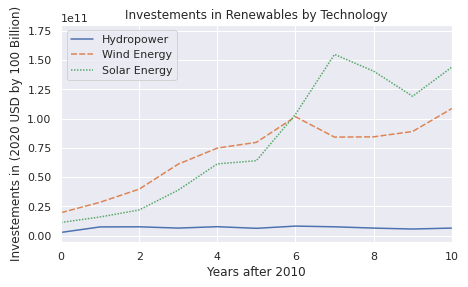
\includegraphics[scale=0.75]{figures/investements_in_renewables.PNG}

{\scriptsize
\begin{figure}[h!]
    \centering
    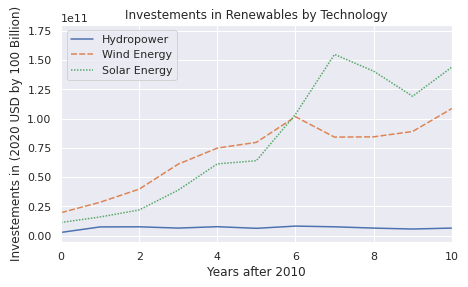
\includegraphics[width=0.6\textwidth]{figures/investements_in_renewables.PNG}
    \caption{Investments in Renewables}

\end{figure}
}


\subsection{Technological Innovation}

Patents Filed for Renewable Technologies - Patents that are filed for Renewable Technologies have been rapidly descending in recent years. Technological innovation could possibly be more important for costs in order to continue to lower and for usage to increase; however, the volume of patients is declining. Figure 6 is very concerning and definitely requires investigation beyond the scope of this paper. Does this information show that tech innovation is stagnating or are there any other explanations? For example, are investors going to choose investments outside of the energy sector (We hear that cryptocurrencies are a big thing right now)?
Innovations in renewable energy encompass new approaches which help to overcome barriers and result in an accelerated deployment of renewables to support the energy transition. Innovative solutions to decarbonize the global energy sector require combining various policy instruments across the whole technology lifecycle, from R&D to market scale-up, as well as the development of new smart technologies, information technology, new types of financial and market instruments, business models, and the engagement of new actors across the energy systems. A number of different things can be done by Governments and Corporations to foster technological innovations and breakthroughs. Putting proper policy incentives in place, base these on long-term perspectives, after all the world cannot switch to renewable energy overnight. Governments should also pursue power system integration, continuing to integrate renewable energies such as Solar and Wind into existing power grids. While integrating these renewable energy sources slowly phase out carbon from different sectors. Innovative policies that provide a framework and balanced support for those researching technological innovation must also be present. These technological advancements go hand in hand with a good financing apparatus, business models, and many different societal changes to promote renewable energy. 

Technological breakthroughs are needed to decrease carbon emissions in the Energy Industry. Even with economically viable and scalable renewable-based solutions available for around two-thirds of the world’s energy supply, population growth and rising energy demand could outpace energy decarbonization without urgent investments in research and development. 


\section{Conclusions}
We found that fossil fuels continue to dominate the energy market, but renewable energy has gained a considerable share. The data trends that this paper covers show that prices of renewable energy have fallen while usage has increased. We were surprised to see that investment in renewable energy is not experiencing much growth. Hydro power is the largest source of renewable energy and investment in this category is somewhat flat. Investment in solar and wind power is surging but these categories are very small portions of the overall energy market. Given how critical it is to replace fossil fuels that are harmful to the environment and human health, it will be worthwhile to explore how to improve investments in Renewable Energy Technological Innovation.

\begin{figure}
    \centering{}
    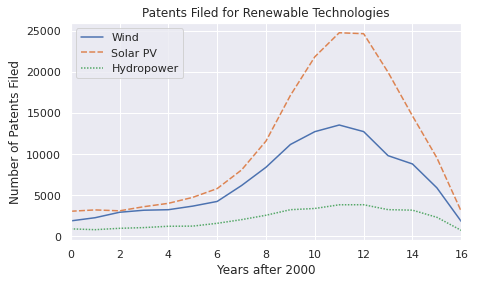
\includegraphics[width=0.6\textwidth]{figures/patents_statistics.PNG}
    \caption{Patents for Renewable Technology}

\end{figure}

\section*{Acknowledgements}
Thank you to the STEM Fellowship Community leaders for making this all possible. Thank you to all the staff, teachers, and mentors that provided guidance, advice, and support during the production of this Data Science research project. 

\bibliography{bibliography}
[1] International Renewable Energy Agency. entitled Renewable Power Generation Costs in 2017. (Max Roser)
\subsection*{}
[2] Frankfurt School-United Nations Environment Programme (UNEP) and the Bloomberg New Energy Finance (BNEF)
\subsection*{}
[3] Hannah Ritchie and Max Roser (2017) - "Air Pollution". Published online at OurWorldInData.org. Retrieved from: 'https://ourworldindata.org/air-pollution' [Online Resource]
\subsection*{}
[4] IRENA (2021), Renewable Power Generation Costs in 2020, International Renewable Energy Agency, Abu Dhabi.
\subsection*{}
[5] IRENA (2018), Renewable Power Generation Costs in 2017, International Renewable Energy Agency, Abu Dhabi
\end{document}





